% !TEX root = main.tex

\section{はじめに}

ムーアの法則が限界を迎え,CPUのコア単位の性能向上はほとんど止まっている.
現在のコンピュータ技術ではCPUに搭載された複数のコアを活用するマルチスレッド処理が主流となっており,マルチスレッドを効果的に使用するソフトウェアやデータ構造などが提案されている.
索引技術においてもその傾向は同様であり,近年ではメニーコアCPU上でのマルチスレッド処理を意識した索引構造が多く提案されている.

代表的な索引構造である\Bptree{}~\cite{book:dbsystem}では,ロックを用いた同時実行制御が行われている.
しかし,マルチスレッド処理においてロックによる同時実行制御は多数の待ちスレッドが発生するため,スケーラビリティが悪化する.
そこで,\Bptree{}を基に構造変更時のロックの占有期間を短くした\Blinktree{}~\cite{tods1981:Lehman}や,楽観的な制御を用いることで\Blinktree{}における読み取り時のロック取得を不要にしたOLFIT~\cite{vldb2001:Cha}などがある.
更に,読み取りおよび書き込みの両方においてロックを取得しないロックフリー索引としてBw木~\cite{book:Bwtree}およびBz木~\cite{book:Bztree}が提案されている.
しかし,これらのロックフリー索引は書き込みの際に競合や多数のスレッドの失敗が発生することによって,マルチスレッド環境では性能が向上していない.
そのため,ロックフリー索引には改善の余地が残されていると考えられる.

本研究では\Bptree{}をロックフリー化させた新たな索引構造である\Bctree{}を提案し,その構造および操作について述べる.
そして提案した索引構造を実装し,Bw木やBz木といったロックフリー索引と比較し,その性能を検証する.

本稿の構成は以下の通りである.
\Sec{\ref{sec:relatedwork}}では,ロックフリー索引の関連研究としてBw木およびBz木について概説する.
次に,\Sec{\ref{sec:bc_tree_structure}}で\Bctree{}の構造について説明し,\Sec{\ref{sec:bc_tree_operation}}で\Bctree{}の操作について述べる.
最後に,\Sec{\ref{sec:conclusion}}で本稿のまとめと今後の方針を述べる.

\section{関連研究}
\label{sec:relatedwork}

近年では,ロックを取得しないロックフリー索引に対して注目が集まっている.
本節では関連研究として,ロック期間の短縮を狙った索引である\Blinktree{}と楽観的制御により読み取り時のロック取得を不要にしたOLFIT,そして代表的なロックフリー索引であるBw木およびBz木について説明する.

\subsection{\Blinktree{}}

% TODO:記述

\subsection{OLFIT}

% TODO:記述

\subsection{Bw木}

Bw木は,直感的にはロックフリーの単方向連結リストと\Bptree{}を組み合わせた索引構造である.
更新内容が記述された差分レコード(delta record)をノードの前に連結リストとして挿入し,索引に対する全ての更新を表す.
差分レコードのリストが一定以上の長さを持つとき,ノードの統合走査が行われ,統合後は\Bptree{}のノードと同様のものが生成される.
また,単一のCAS命令を用いてノードの間のポインタをインストールできるようメモリ内のデータ構造を設計することにより,木のロックフリー化を実現している~\cite{book:DatabaseInternals}.

Bw木が持つ他の木と異なる点として,差分レコードの他にマッピングテーブルがある.
マッピングテーブルはノード間のリンクを仮想化し,メインメモリ上の差分更新を可能とする.
各ノードは自身の子ノードや兄弟ノードへのポインタを直接持つ代わりにマッピングテーブル上のID(logical page ID, LPID)を持つ.
つまり,マッピングテーブルを用いてLPIDを実際のポインタへと変換することでノードを辿る.

\subsection{Bz木}

Bz木は,\Bptree{}の葉ノード内部にロックフリーの固定長配列を持つ索引構造である.
Bz木は,Bz木の根を示すルートポインタと,複数の内部ノードと葉ノードからなる.
ルートポインタが木の根となるノードへのポインタを持ち,根ノードおよび中間ノードなどの内部ノードが子となる内部ノードまたは葉ノードへのポインタを持つ.
Bz木は単一のCAS命令ではなく,メモリ上の複数のワードを対象とするmulti-word compare-and-swap(MwCAS)命令を用いて木のロックフリー化を実現している.

Bz木の各ノードにはヘッダ,メタデータ,レコードが格納されている.
ヘッダにはステータスワードというフィールドが格納されており,ステータスワードはCAS命令や構造変更操作の制御,ノード内のレコード数などノード更新時に必要な情報を格納している.
Bz木はノードに対する書き込みおよび構造変更操作をステータスワードを更新することによってロックフリーに実現している.

\section{\Bctree{}の構造}
\label{sec:bc_tree_structure}

% Bc木の概要
\Bctree{}はBw木とBz木を組み合わせたロックフリー索引である.
\Bctree{}の概形を\Fig{\ref{fig:bc_tree-structure}}に示す.
木の論理的な構造は\Blinktree{}に則っており,各ノードが同じ階層の右兄弟への参照リンクを持つ.
各ノードへの参照はマッピングテーブルを用いた間接参照を採用し,マッピングテーブル内の物理ポインタを差し替えることでそのノードへの参照を一括で変更する.

\begin{figure*}[t]
    \centering
    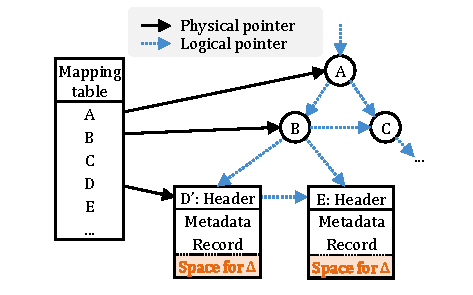
\includegraphics{./figures/Bc-structure.pdf}
    \caption{\Bctree{}の概形}
    \label{fig:bc_tree-structure}
\end{figure*}

% Bc木ノードの説明
\Bptree{}と同様に,\Bctree{}は索引層およびデータ層によって構成される.
索引層のノード(中間ノード)は分割キーと子ノードへのポインタの組を格納し,木の下方への検索を補助する.

各ノードの領域はimmutable領域とmutable領域に分けられる.
immutable領域はノードヘッダおよびソート済みのレコードを格納する.
ヘッダはimmutable領域の情報を管理し,構造変更時のみその値が変更される.
mutable領域はステータスワードの格納と差分レコードを挿入するための書き込みバッファの役割を果たす.
ステータスワードはmutable領域の情報を管理し,ノードの現在の状態や残容量などを管理する.
各ノードへ構造変更操作を行う際は,構造変更後のノードから構造変更前のノードへ物理リンクを張り,古いノードへの参照を可能にする.
なお,古いノードは構造変更が済み次第,ガベージコレクションへ追加され,他のスレッドから参照されないことが保証された時点で削除される.

% Bc木の利点
\Bctree{}はBw木およびBz木でそれぞれボトルネックとなる箇所を以下の通りに克服している.
Bw木ではデルタレコードによって更新を実現しているが,差分レコードの探索はランダムアクセスでありキャッシュヒット率が低い.
そこでBz木のノード内の書き込みバッファを採用することで,Bw木で発生していたデルタレコードによるキャッシュミスを削減している.
次に,Bz木は差分レコードの書き込みおよび対応するレコードメタデータの更新をMwCAS命令を用いたステータスワードの更新によって実現している.
また,同時に発生した構造変更操作を検知するためにステータスワードが変更されていないことをMwCAS命令を用いて確認している.
このようにBz木では,各操作がステータスワードに強く依存している.
そこで,差分レコード用の領域を確保する際にステータスワードを更新し,差分レコードの書き込みおよびメタデータの挿入を完了するといった手法でステータスワードの更新するフィールドを少なくする.
また,Bw木のマッピングテーブルを採用することで,構造変更後のノードに他のスレッドが到達できる.
以上により,Bz木のようなステータスワードに対する強い依存を軽減している.

\section{\Bctree{}の操作}
\label{sec:bc_tree_operation}

本節では,\Bctree{}のノード操作および構造変更操作について述べる.

\subsection{ノード操作}

\Bctree{}は以下の読み取りおよび書き込み操作をサポートする.

\subsubsection{書き込み}

% 書き込み操作の概要
書き込み操作はキーとペイロードを差分レコード領域に挿入する操作である.
キーが属する書き込み先の葉ノードを根ノードから二部探索により特定する.
挿入先の葉ノードに到達後,その葉ノードの差分レコード領域に値を挿入する.

% 書き込み操作の具体的な手順
書き込み操作は差分レコード領域の予約とレコード挿入および可視化の2ステップで行われる.
\Fig{\ref{fig:bc_tree_insertion}}に\Bctree{}における差分レコード挿入を示す.
ノードヘッダにはmutable領域の状態を表すステータスワードを用意し,この中のレコード数と使用済みブロックサイズを加算することで差分レコード用の領域を予約する.
確保した領域へ差分レコードを書き込み,対応するレコードメタデータの値を更新することで挿入処理を完了する.

\begin{figure}[t]
    \centering
    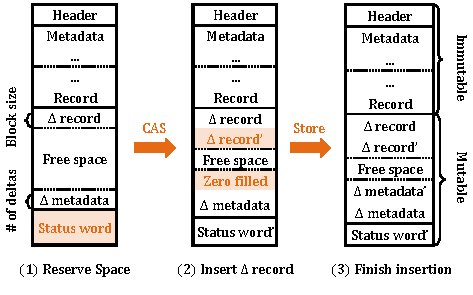
\includegraphics{./figures/Bc-insertion.pdf}
    \caption{\Bctree{}における差分レコードの挿入}
    \label{fig:bc_tree_insertion}
\end{figure}

% 書き込みができない場合の対処
以上の書き込み操作によって差分レコードを挿入していくが,挿入後の差分レコードの総数またはノード容量のしきい値を越える場合,差分レコードの統合操作または構造変更操作が行われる.
しきい値の確認はステータスワードの更新時に行われ,しきい値を越えた場合はレコードの書き込み後に統合操作,構造変更操作いずれかの操作を行うか判定する.

% Bc木の書き込み操作の特徴
書き込み処理は基本的にロックフリーに動作する.
書き込み同士の競合は基本的にステータスワードで解決され,差分レコード用領域の予約はCAS命令によって順序付けられる.

\subsubsection{読み取り}

% 読み取り操作の概要
読み取り(Read)は与えられた対象キーのペイロード返す操作である.
対象キーが与えられたとき,根ノードからの二部探索によりキーが属する葉ノードに到達する.
葉ノードに到達した後は,葉ノード内の差分レコードを線形探索とmutableレコードの二部探索の2ステップで読み取り操作を行う.
対象キーが存在している場合には,対応するペイロードを読み返す.
対象キーが存在していない場合には,存在していない旨を返す.
また,\Bctree{}は始点キーおよび終点キーを指定し,そのキー範囲内の全てのペイロードを返す範囲読み取り(Scan)操作も行う.

% 読み取り操作の具体的手順
最新の値は差分レコード領域に書き込まれるため,まずmutable領域を線形探索し,一致するキーがあるか確認する.
このとき,差分レコードの数はステータスワードから読み取り,差分レコードが可視化されていなければスキップする.
差分レコード中に対象のレコードが存在しなければ,ノードヘッダからimmutableレコードの数を読み取り,二部探索によって対象キーの有無を確認する.
先頭ノードが統合操作の途中である場合には,差分レコードを読み終わった時点で物理ポインタをたどり古いノードへ移動し,同様の2ステップを古いノード上で行う.

% Bc木における読み取り操作の特徴
読み取り処理はwait-freeに動作する.
読み取り処理は一切のノード状態のを変更しないため,読み取った状態に応じて手続きを選択する処理が止まることはない.

\subsection{構造変更操作}

\Bctree{}は以下の統合,分割およびマージをサポートする.
構造変更操作を始める前に,新たなノードをマッピングテーブルに挿入することで,他のスレッドの待ち時間を削減する.

\subsubsection{統合}

% 統合操作の概要と具体的な手順
統合操作は差分レコードの数またはノードの容量がそれぞれのしきい値を越えた場合,差分レコードとimmutableレコードをソートしてimmutable領域に反映する操作である.
\Fig{\ref{fig:bc_tree_consolidastion}}に\Bctree{}における統合操作を示す.
統合が必要になった場合,新たなノード領域を用意する.
そして,古いノードのステータスワード更新後,ノードヘッダの情報から統合後に必要なimmutable領域を計算する.
次に,新たなノードにおいてステータスワードを含むヘッダ情報のみを更新した後,新規ノードとしてマッピングテーブル上の参照を更新する.
その後,古いノード上の差分レコードをimmutableレコードへ反映させつつ,新たなノードへレコードをコピーする.
最後に,統合後の状態でノードヘッダを更新し,ステータスワードをCAS命令を用いて更新する.
この間に発生した書き込み操作は新規ノードのmutable領域で受け付ける.
これにより統合操作の間も,読み取り操作は新規レコードのmutable領域,統合前のノードのmutable領域およびimmutable領域の順でレコードを確認することで読み取り操作を実行できる.

\begin{figure}[t]
    \centering
    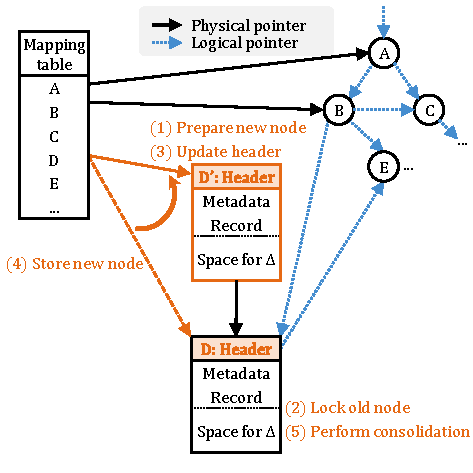
\includegraphics{./figures/Bc-consolidate.pdf}
    \caption{\Bctree{}における統合操作}
    \label{fig:bc_tree_consolidastion}
\end{figure}

\subsubsection{分割}

% 分割操作の概要
分割操作では対象ノードをロックした後,レコードコピーを始める前に分割したノードを用意しマッピングテーブルに挿入する.
これを実現するために,各ノードは自身の分割キーの位置を統合および分割操作のたびに記録する.

% 分割操作の具体的な手順
分割したノードの挿入後,統合操作と同様の手続きでレコードをコピーする.
分割時には,古いノードの分割キー未満の全てのレコードを左ノードにコピーする.
残りのレコード,すなわち分割キー以上の全てのレコードは右ノードにコピーする.
レコードのコピー後は,親ノードに右分割ノードへのリンクを挿入することで分割操作が完了する.
このとき,中間ノードにおけるCPUキャッシュ効率を高めるために,親ノードへはリンクの情報のみを挿入し,反映は親ノードの統合操作時に行う.

% 分割キーについての注意
分割キーはimmutableレコードから決定される.
つまり差分レコードは考慮されないため,分割操作時に片方のノードにレコードの偏りが発生しうる.
前述した通り,分割操作前にノードを用意するため,immutable領域および対応するメタデータ数は余裕を持って確保しておく必要がある.
そのため,差分レコードが片方のノードに集中し,その分のスペースがもう片方のノードで使用されない,未使用なimmutable領域が残る可能性がある.

\section{おわりに}
\label{sec:conclusion}

本稿では,\Bptree{}をロックフリー化させた新たな索引構造\Bctree{}を提案し,その構造および操作を紹介した.
今後は提案した索引構造を実装し,ノードのレコードを他のノードとつなぎ合わせるようなマージ操作など,他の操作を実装する.
また,近年提案されているBw木やBz木といったロックフリー索引との性能を比較検証する.